
\section{Geschichte}

Die Entwicklung der Augmented-Reality-Technologie geht auf die 1960er Jahre zurück, als der Informatiker Ivan Sutherland das erste kopfgetragene Display erfand. Dieses bahnbrechende Gerät, das auch als “Sword of Damocles” bezeichnet wurde, ebnete den Weg für tragbare Computerschnittstellen, obwohl es keine echten AR-Funktionen bot \cite{Sutherland1968AHT}. Nicht lange danach, 1975, gründete Myron Krueger den Videoplace, ein Labor für künstliche Realität. Dieser Raum reagierte auf die Bewegungen und Aktionen der Benutzer und machte Brillen oder Handschuhe überflüssig \cite{Videoplace}.

\vspace{1cm}

\begin{figure}[ht!]
    \centering
    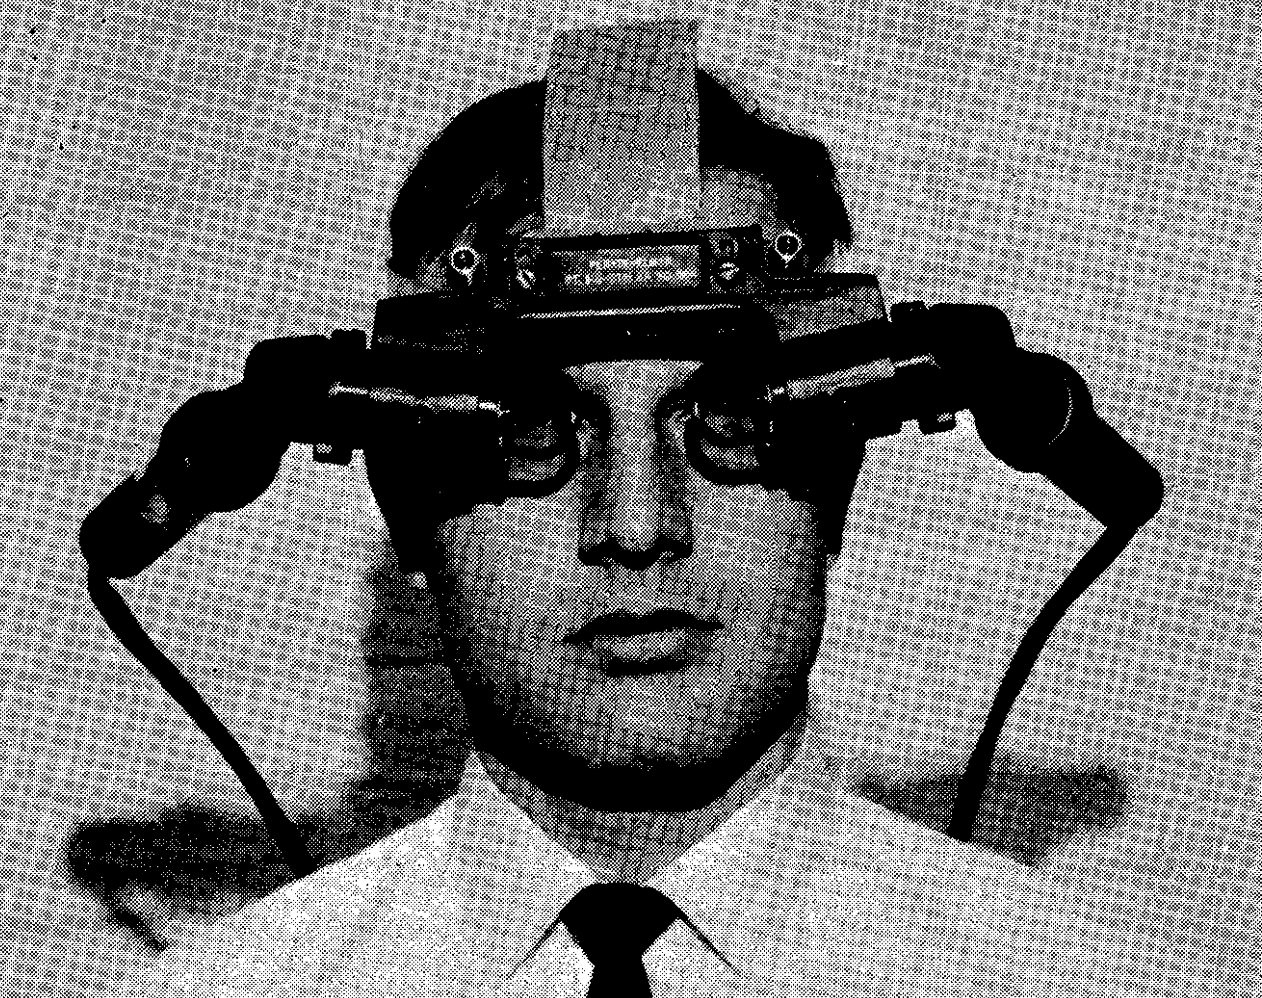
\includegraphics[width=0.6\textwidth]{attachments/Sutherland_1.png}
    \caption{Die Optik des Head-Mounted Displays (HMD)} \cite{Sutherland1968AHT}
\end{figure}


Tatsächlich wurde der Begriff “Augmented Reality” erst 1990 von Thomas P. Caudell, einem ehemaligen Forscher bei Boeing, eingeführt \cite{Lee2012AugmentedRI}. Im Jahr 1992 stellte Louis Rosenburg vom Armstrong Research Lab der United States Air Force “Virtual Fixtures” vor, eines der ersten voll funktionsfähigen Augmented-Reality-Systeme \cite{rosenberg1992use}.

\begin{figure}[ht!]
    \centering
    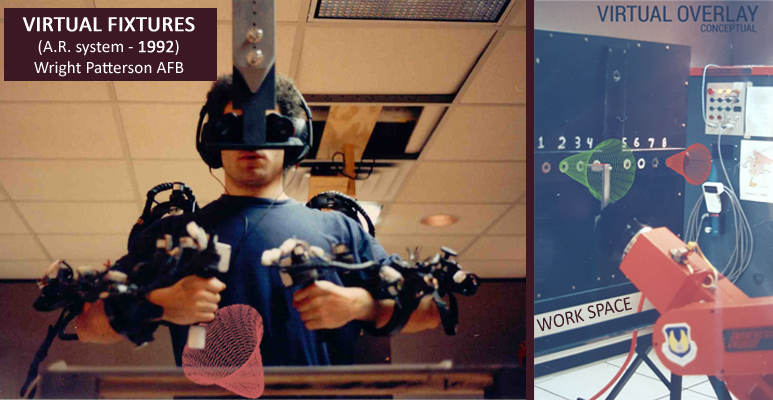
\includegraphics[width=0.7\textwidth]{attachments/Rosenburg.jpg}
    \caption{Dr. Louis Rosenberg trägt ein Oberkörper-Exoskelett} \cite{rosenberg1992use}
\end{figure}

\newpage 

Weitere Entwicklungen in den späten 90er Jahren waren die Definition des Realitäts-Virtualitäts-Kontinuums von Paul Milgram und Fumio Kishino im Jahr 1994, das sich von der realen Umgebung zur virtuellen Umgebung erstreckt. Augmented Reality (AR) und Virtual Reality (VR) liegen dazwischen, wobei sich AR zur realen Welt und VR zur virtuellen Welt neigt  \cite{Milgram94a}. Ronald Azumas Studie von 1997 über AR ist ein weiterer wichtiger Meilenstein, der eine allgemein akzeptierte Definition der Technologie liefert. Azuma definierte AR als die Integration von realen und virtuellen Umgebungen mit 3D-Registrierung und Echtzeit-Interaktivität \cite{Azuma1997ASO}. Im Jahr 2000 brachte Hirokazu Kato das AR ToolKit auf den Markt, eine Open-Source-Softwarebibliothek, die die Entwicklung von AR-Softwareanwendungen durch eine Video-Tracking-Technologie revolutionierte, die virtuelle Grafiken über die physische Welt legt \cite{ARTooLKIT}.

In den frühen 2010er Jahren begannen grosse Technologieunternehmen in die AR-Branche einzusteigen. So stellte Google 2012 seine Google Glass vor, eine Augmented-Reality-Brille, die den Nutzern immersive Erfahrungen bietet \cite{Google_for_Developer_2012}. Im Jahr 2015 kündigte Microsoft Windows Holographic und das HoloLens-Headset für Augmented Reality an. Das Headset verschmolz hochauflösende “Hologramme” mit der physischen Welt \cite{Tech_Discussion_2015}. Im Jahr 2016 wurde die Technologie leichter zugänglich, als Niantic Pokémon Go für iOS und Android veröffentlichte. Die mobile AR-App erfreute sich grosser Beliebtheit und steigerte die Attraktivität von AR-Spielen \cite{Bond_2016}. Darüber hinaus hatte der Aufstieg mobiler AR-Apps einen bemerkenswerten Einfluss auf andere Branchen wie den Einzelhandel. Im Jahr 2017 brachte IKEA seine Augmented-Reality-App IKEA Place auf den Markt, die es den Nutzern ermöglicht, sich vor dem Kauf von Möbeln zu Hause eine Vorschau anzusehen \cite{IKEA_2017}. Im Jahr 2023 schliesslich kündigte Apple das Apple Vision Pro an, ein Augmented-Reality-Headset, das die reale und die digitale Welt “nahtlos” miteinander verschmelzen lässt und den neuesten Fortschritt in der AR-Technologie markiert \cite{Apple}.

\vspace{1cm}

\begin{figure}[ht!]
    \centering
    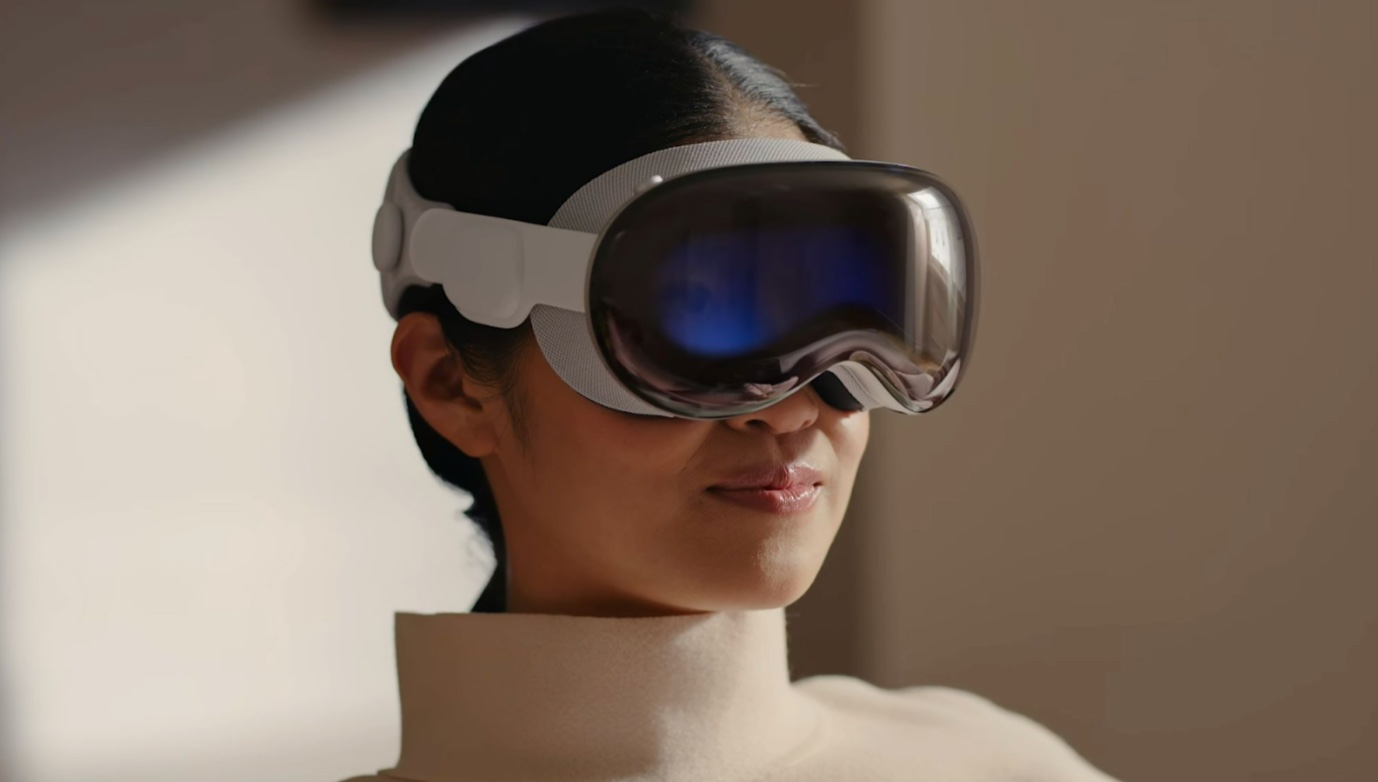
\includegraphics[width=0.7\textwidth]{attachments/Vision_1.jpeg}
    \caption{Apple Vision Pro Gerät} \cite{Apple}
\end{figure}

\begin{figure}[ht!]
    \centering
    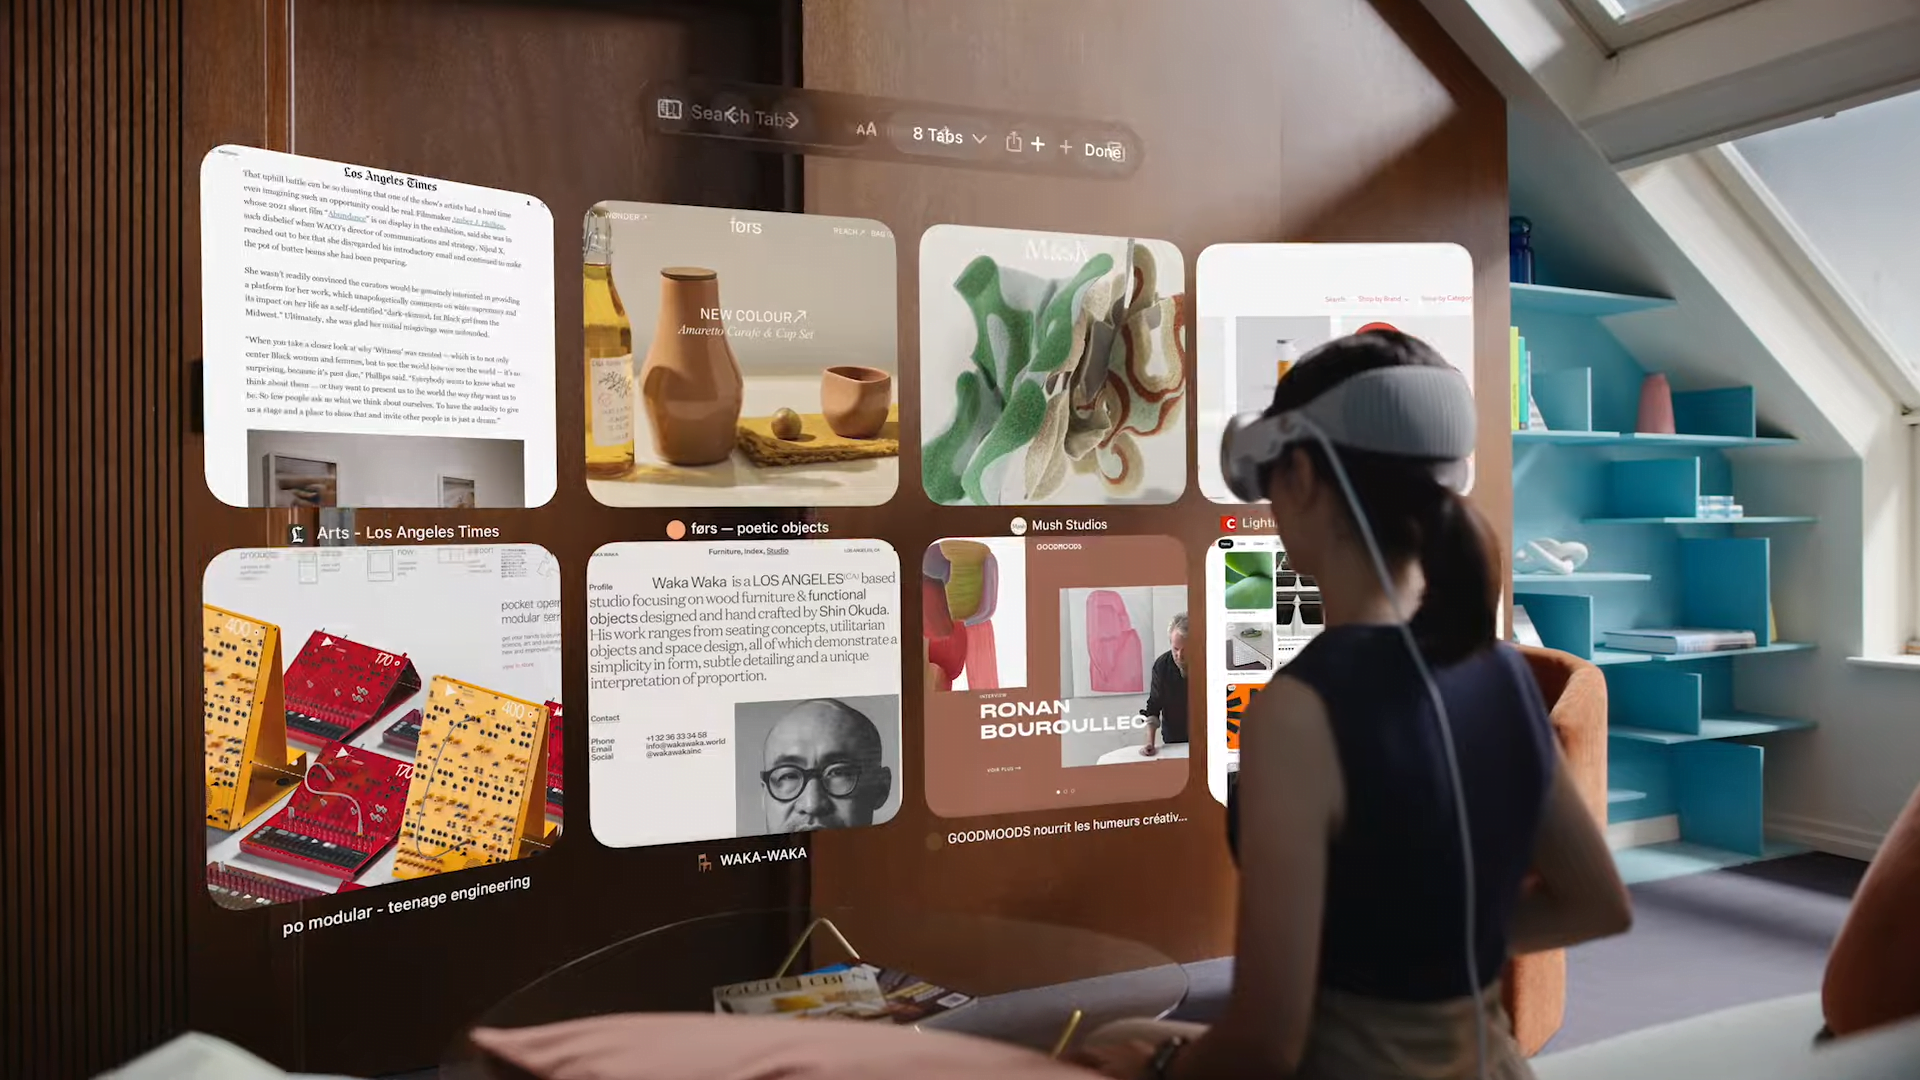
\includegraphics[width=0.7\textwidth]{attachments/Vision_2.png}
    \caption{Apple Vision Pro Software in Verwendung} \cite{Apple}
\end{figure}
